%% This is file `elsarticle-template-2-harv.tex',
%%
%% Copyright 2009 Elsevier Ltd
%%
%% This file is part of the 'Elsarticle Bundle'.
%% ---------------------------------------------
%%
%% It may be distributed under the conditions of the LaTeX Project Public
%% License, either version 1.2 of this license or (at your option) any
%% later version.  The latest version of this license is in
%%    http://www.latex-project.org/lppl.txt
%% and version 1.2 or later is part of all distributions of LaTeX
%% version 1999/12/01 or later.
%%
%% The list of all files belonging to the 'Elsarticle Bundle' is
%% given in the file `manifest.txt'.
%%
%% Template article for Elsevier's document class `elsarticle'
%% with harvard style bibliographic references
%%
%% $Id: elsarticle-template-2-harv.tex 155 2009-10-08 05:35:05Z rishi $
%% $URL: http://lenova.river-valley.com/svn/elsbst/trunk/elsarticle-template-2-harv.tex $
%%
\documentclass[preprint,authoryear,12pt]{elsarticle}

%% Use the option review to obtain double line spacing
%% \documentclass[authoryear,preprint,review,12pt]{elsarticle}

%% Use the options 1p,twocolumn; 3p; 3p,twocolumn; 5p; or 5p,twocolumn
%% for a journal layout:
%% \documentclass[final,authoryear,1p,times]{elsarticle}
%% \documentclass[final,authoryear,1p,times,twocolumn]{elsarticle}
%% \documentclass[final,authoryear,3p,times]{elsarticle}
%% \documentclass[final,authoryear,3p,times,twocolumn]{elsarticle}
%% \documentclass[final,authoryear,5p,times]{elsarticle}
%% \documentclass[final,authoryear,5p,times,twocolumn]{elsarticle}

%% if you use PostScript figures in your article
%% use the graphics package for simple commands
%% \usepackage{graphics}
%% or use the graphicx package for more complicated commands
\usepackage{graphicx}
%% or use the epsfig package if you prefer to use the old commands
%% \usepackage{epsfig}

%% The amssymb package provides various useful mathematical symbols
\usepackage{amsmath,amssymb,amstext} % Lots of math symbols and environments
%% The amsthm package provides extended theorem environments
%% \usepackage{amsthm}

%% The lineno packages adds line numbers. Start line numbering with
%% \begin{linenumbers}, end it with \end{linenumbers}. Or switch it on
%% for the whole article with \linenumbers after \end{frontmatter}.
%% \usepackage{lineno}

%% natbib.sty is loaded by default. However, natbib options can be
%% provided with \biboptions{...} command. Following options are
%% valid:

%%   round  -  round parentheses are used (default)
%%   square -  square brackets are used   [option]
%%   curly  -  curly braces are used      {option}
%%   angle  -  angle brackets are used    <option>
%%   semicolon  -  multiple citations separated by semi-colon (default)
%%   colon  - same as semicolon, an earlier confusion
%%   comma  -  separated by comma
%%   authoryear - selects author-year citations (default)
%%   numbers-  selects numerical citations
%%   super  -  numerical citations as superscripts
%%   sort   -  sorts multiple citations according to order in ref. list
%%   sort&compress   -  like sort, but also compresses numerical citations
%%   compress - compresses without sorting
%%   longnamesfirst  -  makes first citation full author list
%%
%% \biboptions{longnamesfirst,comma}

% \biboptions{}

\usepackage{setspace}
\doublespacing

\journal{Annals of Nuclear Energy}

\begin{document}
\begin{frontmatter}

%% Title, authors and addresses

%% use the tnoteref command within \title for footnotes;
%% use the tnotetext command for theassociated footnote;
%% use the fnref command within \author or \address for footnotes;
%% use the fntext command for theassociated footnote;
%% use the corref command within \author for corresponding author footnotes;
%% use the cortext command for theassociated footnote;
%% use the ead command for the email address,
%% and the form \ead[url] for the home page:
%% \title{Title\tnoteref{label1}}
%% \tnotetext[label1]{}
%% \author{Name\corref{cor1}\fnref{label2}}
%% \ead{email address}
%% \ead[url]{home page}
%% \fntext[label2]{}
%% \cortext[cor1]{}
%% \address{Address\fnref{label3}}
%% \fntext[label3]{}

\title{Reliability analysis of digital feedwater regulating valve controller system using semi-Markov process model}

%% use optional labels to link authors explicitly to addresses:
%% \author[label1,label2]{}
%% \address[label1]{}
%% \address[label2]{}

\author{Arun Veeramany and Mahesh D. Pandey}

\address{Department of Civil and Environmental Engineering, University of Waterloo \\
Waterloo, Ontario, N2L 3G1, Canada \\ aveerama@uwaterloo.ca}

%\maketitle


\begin{abstract}
A semi-Markov process model is developed for the reliability analysis of main feedwater valve (MFV) controller system used for regulating the water level in a power plant steam generator. This case study demonstrates the general application of semi-Markov process model for digital instrumentation and control systems. The NUREG-CR/6942 technical report proposed a Markov state transition model for the MFV system as part of a Probabilistic Risk Assessment (PRA) of Digital Feedwater Control System (DFWCS). The proposed model extends the Markov model to allow the use of non-exponential distribution in the time to next output of the controller system responsible for maintaining the water level. Through the concept of mission reliability,  the paper is able to demonstrate that by assuming a non-exponential profile for transition times, it is possible to take hardware and software aging in to account.  

\end{abstract}



\begin{keyword}
%% keywords here, in the form: keyword \sep keyword
Digital Instrumentation and Control \sep Reliability \sep Semi-Markov
%% PACS codes here, in the form: \PACS code \sep code

%% MSC codes here, in the form: \MSC code \sep code
%% or \MSC[2008] code \sep code (2000 is the default)

\end{keyword}

\end{frontmatter}

\section{Introduction}

Digital control and protection systems are installed in new nuclear power plants (NPP) and as part of upgrades to older plants. There could be random hardware failures in these systems, but random software faults are less likely to occur \citep{Chu2010a}. While hardware failures can be modeled probabilistically, software failures can also be modeled in the same way assuming that the faults caused in software are due to an underlying cause in the digital system. The failure of an I\&C system could potentially lead to core damage or release of radioactive substances  \citep{Shi2010}.

\subsection{Need for reliability analysis of I\&C systems}
Reliability is a result of features like fault tolerance, fault coverage, fail safe, redundancy, defense-in-depth and diversity of components. Digital system reliability models either account for hardware and software failures separately or take both in to consideration in a single model. Software failures could potentially impact the performance of mitigating systems. Certain failure modes could arise due to software which was not originally considered for analog systems \citep{Chu2010a}. Hence digital system reliability modelling is an area of important research. 

\subsection{Literature}
The technical report by \cite{NUREG6901} explored various methods available for system reliability evaluation of digital instrumentation and control (I\&C)  systems. Static fault tree and event tree approaches were considered obsolete due to the inherent inability of these methods to tackle ``dynamic interaction'' between  digital systems and rest of the plant processes. An example of such an interaction is a competition between two tasks to get hold of a digital controller's resources.  Deadlock could be a situation when two threads wait for each other to release resources they are in control of. Starvation is a situation where a low priority thread might have to wait indefinitely for the controller's time slice. Hence temporal interactions could lead to dynamic situations and these can be handled well using state transition methods by branching different situations as distinct states. Despite the provisions for specialized dependency gates, the dynamic fault tree (DFT) method \citep{DurgaRao2009872} has the shortcoming that the generated cutsets might change as the system evolves in time. 


The dynamic flowgraph methodology, DFM \citep{AlDabbagh20101202} is another alternative for modelling reliability of digital I\&C systems. It takes the directed graph approach with decision tables for state transitions, edges for failure dependencies and nodes for variables ($.e.g.,$ Water level, Valve position). Nodes can have discrete states ($e.g.,$ High, Stationary, Low). The decision table construction involves all possible mappings of variables and corresponding states (e.g., Water level high and valve open).  The mapping must also account for various switching actions for backup solutions. \cite{Yau1995} demonstrated the use of DFM for a digital flight control system where 9 input variables with 5 states each led to $5^9$ rows in the decision table. The paper worked around the problem by using equations of motion and control laws thus bypassing the construction and lookup of the decision table. Hence decision table construction could potentially encounter a dimensionality problem and modelling would not adhere to a universal solution though it has the ability to model multiple top events. Stochastic petri nets \citep{Kleyner2010606} is also a graph theoretic approach whose quantification can be done using simulation. These models can be converted to fault trees, but size of the model and simulation speed could severely prohibit its usage for digital I\&C systems.



Another technical report by \cite{NUREG6942} focused exclusively on reliability modelling of digital I\&C systems for nuclear reactor probabilistic risk assessments. Markov models were developed for various controllers and computer systems of the DFWCS. These include the main feedwater regulating valve (MFV) controller, the bypass feedwater regulating valve (BFV) controller, the feedwater pump (FP) controller, the pressure drop indicator (PDI) controller, power source of these controllers and finally the main and its backup computers.   This report was at large a proof-of-concept for the use of Markov models for digital systems. The state space for the models were elaborately developed and then reduced according to state reduction principles for practical applications. \cite{Aldemir20101011} refined and quantified some of these models by generating Markov transition rates using fault injection techniques. Such techniques in software testing widen the scope of test data by introducing deliberate faults in the system. 

Markov models are able to predict future failures while considering failure dependencies and can accommodate both hardware and digital interaction. However, Markov models  assume only constant transition rates leading to the assumption that the time spent in any state can follow only the exponential distribution.  A system involving complex interactions between hard-wired analog and software controlled digital subsystems could be subjected to human, software, electrical, mechanical and electronic failures. Lognormal, Weibull and Gamma distributions to represent time-to-event have been found to be appropriate in different contexts \citep{Vineyard1999139}.


%A broad overview of probabilistic safety assessment for digital I\&C systems in the areas of quality assurance, surveillance testing and I\&C design is given by \cite{LixuanLU2004323}.
%\cite{Clarotti1980} carried out reliability analysis of a computerized nuclear reactor protection system. The paper chose Markov model for the task assuming the following as random variables: time to detectable and undetectable computer failure, time to reactor trip and startup and also the time to detect a detectable failure. The model consisted of eleven states with the aim of evaluating accident probability in the plant. The states were determined based on two minicomputers and the protection and self-checking programs running on them.


\subsection{Proposed approach}
A water level controller valve could be subject to high failure rates due to surge voltages during startup or shutdown and a fairly constant failure rate at any random running time. With this rationale, the present paper assumes that a Weibull distribution is suitable to model the time to a send a previous valid output to the valve. In order to achieve this ability to consider a non-exponential holding time distribution in the model, the semi-Markov process model is applied for the reliability analysis of digital feedwater regulating valve controller.
The idea of applying semi-Markov process model to incorporate the effect of aging related degradation of pipes in the nuclear industry has earlier been explored by \cite{Veeramany2011}.


Markov model requires continuous plant state information to generate the transition rates required as inputs. The semi-Markov process model is also subject to this inhibitive requirement. Further disadvantage is the difficult learning curve for an analyst. This hindrance can be negated to an extent by the use of simple visual interfaces.


\subsection{Organization}

The paper is organized as follows. Section \ref{sec:MFVSystemDesc} describes the digital controller system. 
Section \ref{sec:DICMarkovModel} describes the Markov model of the system. The semi-Markov process model is reviewed in Section \ref{sec:SMPModel}. Section \ref{sec:SMPDigitalSystems} develops the semi-Markov version of the controller reliability study. Markov results are compared against the semi-Markov results in Section \ref{sec:DICResults} before concluding the paper in Section \ref{sec:DICConclusion}.


\section{The digital feedwater regulating valve controller system}
\label{sec:MFVSystemDesc}

\subsection{Problem}
\begin{figure}[h!] \centering
  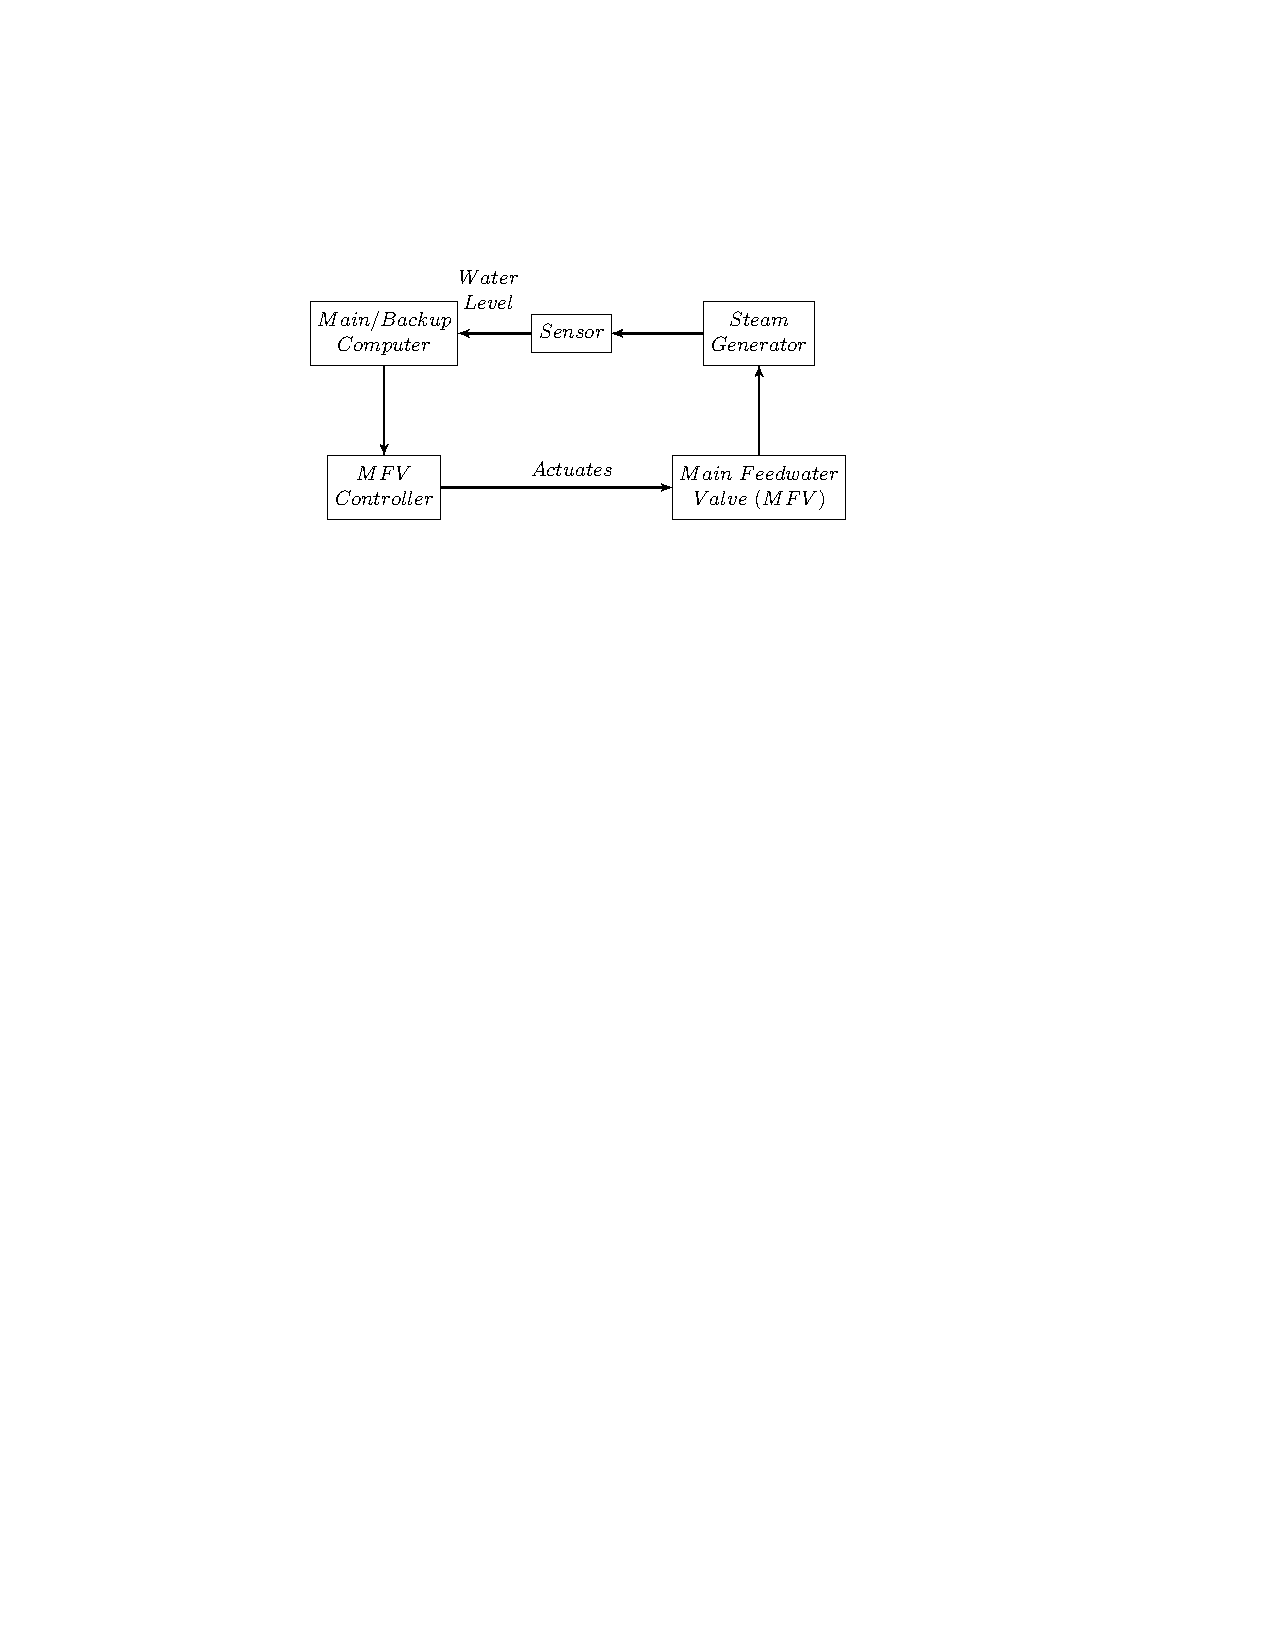
\includegraphics[scale=0.9]{MFVLayout}
  \caption{Schematic of the digital feed water control system (DFWCS).\label{fig:MFVLayout}} 
\end{figure}
The present paper is a semi-Markov extension of one of the feedwater controller Markov models from \cite{Aldemir20101011}. The digital feed water control system (DFWCS) shown in Figure \ref{fig:MFVLayout} is responsible for regulating  water level in the steam generator. A water level sensor outputs  level to the computer. The computer then determines the amount by which the valves need to be repositioned so as to adjust the water flow speed. This information is sent in the form of a signal to the controller. Accordingly, the controller actuates the main feedwater regulating valve (MFV) to optimize the water flow. Apart from MFV, there are other controllers and actuating devices as part of the DFWCS. The focus of this paper is to analyze the reliability of the MFV controller system based on its output to the valve. There is a finite probability of the valve getting stuck in its maximum or minimum flow position due to an erroneous output from the controller. It is also possible that the controller sends an arbitrary or random output to the valve. These could be due to a processing error or an internal problem in the computer. In these abnormal cases the controller feeds a valid previous output to the valve. This situation is termed as the failure of the controller system.






\subsection{Markov analysis}
\label{sec:DICMarkovModel}


\begin{figure}[h!] \centering
  \includegraphics[scale=0.8]{ControllerStateSpace}
  \caption{State space for Main Feedwater regulating Valve (MFV)\citep{Aldemir20101011}.\label{fig:ControllerStateSpace}} 
\end{figure}

The model proposed by \cite{Aldemir20101011} based on \cite{NUREG6942} has five states as shown in Figure \ref{fig:ControllerStateSpace}. The system initially begins operation in state 1. In this state, the controller receives correct output from the computer and sends it to the valve. The system moves to state 2,4 or 5 when the output is too low, high or arbitrary respectively. It is assumed that these states do not lead back to the correct output, instead move on to state 3 where a valid previous output is sent to the valve. For modelling purposes, state 3 is an absorbing state representing system failure. As per this model, there is a transition from state 1 to state 3 in which case an internal problem with the computer is recognized by the controller and a previous output is sent to the valve. The literature also suggests that there are circumstances when the controller fails to sense the failure of the computer and hence sends arbitrary output to the valve.




\begin{table}[!h]\centering
\caption{Sample Markov transition rates for the controller system. \citep{Aldemir20101011}\label{tbl:DICMarkovRates}}
\begin{tabular}{l l l l l}
\hline
\multicolumn{4}{c}{State Transition} & Transition Rate ($hr^{-1}$)\\
\hline
$\lambda_{12}$	&	 Correct Output & $\rightarrow$ & Output Low	&	2.55 \text{x} $10^{-7}$	\\
$\lambda_{13}$	&	 Correct Output & $\rightarrow$ & Previous Output	&	4.2 \text{x} $10^{-5}$	\\
$\lambda_{14}$	&	 Correct Output & $\rightarrow$ & Output High	&	5.5 \text{x} $10^{-8}$	\\
$\lambda_{15}$	&	 Correct Output & $\rightarrow$ & Arbitrary Output	&	5.5 \text{x} $10^{-8}$	\\
$\lambda_{23}$	&	 Output Low & $\rightarrow$ & Previous Output	&	4.2  \text{x} $10^{-5}$	\\
$\lambda_{43}$	&	 Output High & $\rightarrow$ & Previous Output	&	4.2  \text{x} $10^{-5}$	\\
$\lambda_{53}$	&	 Arbitrary Output & $\rightarrow$ & Previous Output	&	4.2  \text{x} $10^{-5}$	\\
\hline
\end{tabular}
\end{table}

Due to lack of field data, \cite{Aldemir20101011} assumed failure rates based on fault injection experiments. The authors claim that these rates listed in Table \ref{tbl:DICMarkovRates} were for demonstrative use only.

The system of differential equations to solve the Markov model is based on the fact that the rate of change of the 
probability  of being in any state $S$ is negatively proportional to the rate at which
the transitions occur outward from $S$ and positively proportional to the rate at which inward transitions occur from other states \citep{Lisnianski2003}.

For example, from Figure \ref{fig:ControllerStateSpace}, it is seen that there are four inward transitions in to state 3  originating from states 1,2,4 and 5 while there is only one transition going out from states 2,4 and 5.


\begin{align}
dp_1(t)/dt & =   -(\lambda_{12} + \lambda_{13} + \lambda_{14} + \lambda_{15}) p_1(t) \nonumber	\\
dp_2(t)/dt & =\lambda_{12} p_1(t)    -\lambda_{23} p_2(t)	\nonumber \\
dp_3(t)/dt & =\lambda_{13} p_1(t) + \lambda_{23} p_2(t) + \lambda_{43} p_4(t) +\lambda_{53} p_5(t) \nonumber \\
dp_4(t)/dt & =\lambda_{14}p_1(t)    -\lambda_{43}p_4(t) \nonumber \\
dp_5(t)/dt & =\lambda_{15} p_1(t)    -\lambda_{53} p_5(t)
\label{eq:DICMarkovEqns}
\end{align}

\begin{figure}[h!] \centering
  \includegraphics[scale=0.8, angle=-90]{MarkovState3}
  \caption{Controller failure probability.\label{fig:MarkovState3}} 
\end{figure}

\subsection{Results}
Solving system of Equations \ref{eq:DICMarkovEqns}, Figure \ref{fig:MarkovState3} plots the probability of being in state 3 and it represents the controller system failure probability. Note that the system could land in state 3 either directly from state 1 or through the other states. 
Out of a year, the operational mission time of the DFWCS is assumed to be 11 months allowing for one month of outage time \citep{NUREG6942}. For  PRA purposes, the usual (default) reference time period is 24h \citep{Aldemir20101011}.
Hence, in this paper, time scale for all the plots is 24h beginning at time zero assuming a system reset.



\begin{figure}[h!] \centering
  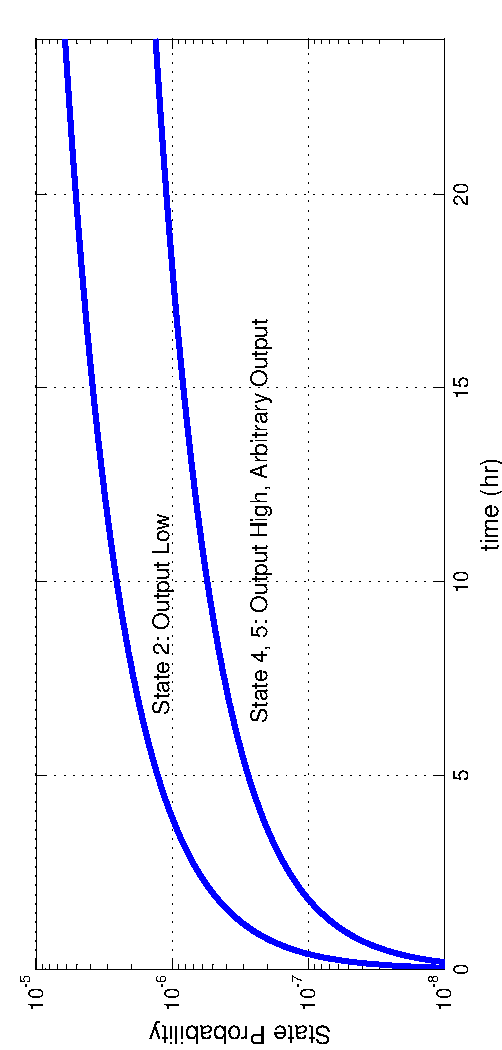
\includegraphics[scale=0.8, angle=-90]{MarkovStates245}
  \caption{Probability of being in states 2,4 and 5.\label{fig:MarkovStates245}} 
\end{figure}


Figure \ref{fig:MarkovStates245} plots the probability of being in states 2, 4 and 5. The state probability of a high or an arbitrary output is the same owing to the same failure rate shared by the respective transitions from the state of correct output. The failure rate of a low output from correct output is lower than that of a high or an arbitrary output. Correspondingly, the state probabilities reflect the trend. However, comparing Figure \ref{fig:MarkovState3} and \ref{fig:MarkovStates245} the probability of a controller failure is higher than being in any of the other states. This can be attributed to the fact that state of previous output is an absorbing state and hence all transitions eventually end in this state.


A direct transition from correct to previous output has higher influence over the controller failure probability than that due to transiting through intermediate steps and reaching the previous output. This is due to relatively larger failure rate for the transition from correct to previous output when compared to the combined failure rates of the alternate paths.



%\section{The Semi-Markov Process Model}
\label{sec:SMPModel}
This project follows the general formulation of the continuous-time discrete-state semi-Markov process model as developed in \cite{HowardA} and \cite{HowardB}. 

Let the model have $N$ states. Let $f_{ij}(t)$ and $F_{ij}(t)$ represent the   $pdf$ and $cdf$ respectively of the event corresponding to the transition from state $i$ to state $j$ at time $t$. 

Assume that the process is in state $i$. From this state, there could be $k$ different states to which the process could transit to in a single step. Also assumed in this model is that all these $k$ possibilities are independent of the occurrence of each other. At a time instant $t$, the process chooses only one state from these choices such that the time to be spent in the current state $i$ is the minimum before instantaneously jumping to the chosen state. The probability that the next state is $j$ and not any other state $k$ reachable from $i$ is given by:
\begin{align}
\label{eq:CompRisk}
c_{ij}(t) =  f_{ij} (t)\prod\limits_{k \ne j} {(1 - F_{ik} (t))} 
\end{align}
For $N$=2, $c_{ij}(t) =  f_{ij} (t)$. The matrix $C(t)=[ c_{ij}(t) ]$ is called the kernel or core of the semi-Markov process model and
\begin{align}
\label{eq:waiting}
w_i(t) = \sum\limits_{j=1}^{N}{c_{ij}(t)}
\end{align}
is called the waiting time distribution for the state $i$. It represents the probability that the process waits in state $i$ for $t$ time units before making a transition. Hence it is an unconditional probability distribution. 
It is assumed that any row $i$ of the kernel $C=[c_{ij}]$ satisfies the condition:
\begin{eqnarray}
\int\limits_0^\infty  { \sum\limits_{j}^{}{c_{ij}(t)} dt \approx 1} 
\label{eq:MREAssumption}
\end{eqnarray}
This assumption assures that there is unit probability that the process
will be in one of the $N$ states of the process at time $t$, given the initial 
state as $i$. The probability that the process does not leave state $i$ by time $t$ is given by:
\begin{align}
\label{eq:staying}
W_i (t) = 1 - \int\limits_0^t {w_i(t)dt} 
\end{align}
The objective of the model is to determine the probability $\phi_{ij}(t)$  of being in each state  $j$ given that the process initially is in a particular state $i$. $\phi_{ij}(t)$  can be determined by solving a system of integral equations:
\begin{align}
{\phi _{ij} (t)} = \delta _{ij} W_i (t) + \sum\limits_k {\int\limits_0^t {c_{ik} (\tau ){\phi _{kj} (t - \tau )}d\tau } } 
\label{CTMRE}
\end{align}
Where $i=j=k=0,1,2,...N-1$.	 


The right hand side of Equation \ref{CTMRE} describes the following probabilities:
\begin{enumerate}
\item	$i=j$ and second term=0: $W_i (t)$ is the probability that the process does not leave state $i$ by time $t$.
\item	$i=j$ and second term not 0: process leaves state $i$ and returns to $i$ by time $t$.
\item	$i \neq j$  and second term $\neq j$ : process leaves state $i$ and reaches state $j$ by time $t$.
\end{enumerate}
The system of equations can alternatively be written in a compact form as a matrix:
\begin{align}
{\phi(t)} = diag(W(t)) + {\int\limits_0^t {C(\tau ){\phi (t - \tau )}d\tau } } 
\label{MatMRE}
\end{align}




\section{Proposed Semi-Markov Process Model}
\label{sec:SMPModel}

\subsection{Analysis}
This paper follows the general formulation of the continuous-time discrete-state semi-Markov process model as developed by \cite{HowardA, HowardB}. 

Let the model have $N$ states. Let $f_{ij}(t)$ and $F_{ij}(t)$ represent the   $pdf$ and $cdf$ respectively of the event corresponding to the transition from state $i$ to state $j$ at time $t$. 

Assume that the process is in state $i$. From this state, there could be $k$ different states to which the process could transit to in a single step. These states could be completion of a repair, further degradation of the system or a failure mode with an underlying failure mechanism. Also assumed in this model is that all these $k$ possibilities are independent of the occurrence of each other. At a time instant $t$, the process chooses only one state from these choices such that the time to be spent in the current state $i$ is the minimum before instantaneously jumping to the chosen state. The probability that the next state is $j$ and not any other state $k$ reachable from $i$ is given by:

\begin{align}
\label{eq:CompRisk}
c_{ij}(t) =  f_{ij} (t)\prod\limits_{k \ne j} {(1 - F_{ik} (t))} 
\end{align}

For $N$=2, $c_{ij}(t) =  f_{ij} (t)$. The matrix $C(t)=[ c_{ij}(t) ]$ is called the kernel or core of the semi-Markov process model and
\begin{align}
\label{eq:waiting}
w_i(t) = \sum\limits_{j=1}^{N}{c_{ij}(t)}
\end{align}
is called the waiting time distribution for the state $i$. It represents the probability that the system waits in state $i$ for $t$ time units before making a transition. Hence it is an unconditional probability distribution. 
It is assumed that any row $i$ of the kernel $C=[c_{ij}]$ satisfies the condition:
\begin{eqnarray}
\int\limits_0^\infty  { \sum\limits_{j}^{}{c_{ij}(t)} dt \approx 1} 
\label{eq:MREAssumption}
\end{eqnarray}
This assumption assures that there is unit probability that the system
will be in one of the $N$ states of the system at time $t$, given the initial 
state as $i$. The probability that the system does not leave state $i$ by time $t$ is given by:
\begin{align}
\label{eq:staying}
W_i (t) = 1 - \int\limits_0^t {w_i(t)dt} 
\end{align}
The objective of the model is to determine the probability $\phi_{ij}(t)$  of being in each state  $j$ given that the system initially is in a particular state $i$. $\phi_{ij}(t)$  can be determined by solving a system of integral equations:
\begin{align}
{\phi _{ij} (t)} = \delta _{ij} W_i (t) + \sum\limits_k {\int\limits_0^t {c_{ik} (\tau ){\phi _{kj} (t - \tau )}d\tau } } 
\label{CTMRE}
\end{align}
Where $i=j=k=0,1,2,...N-1$.	 


The right hand side of Equation \ref{CTMRE} describes the following probabilities:
\begin{enumerate}
\item	$i=j$ and second term=0: $W_i (t)$ is the probability that the process does not leave state $i$ by time $t$.
\item	$i=j$ and second term not 0: process leaves state $i$ and returns to $i$ by time $t$.
\item	$i \neq j$  and second term $\neq j$ : process leaves state $i$ and reaches state $j$ by time $t$.
\end{enumerate}

The system of equations can alternatively be written in a compact form as a matrix:
\begin{align}
{\phi(t)} = diag(W(t)) + {\int\limits_0^t {C(\tau ){\phi (t - \tau )}d\tau } } 
\label{MatMRE}
\end{align}

Given that the system started its operation in state $i$ and that state $j$ is the only absorbing state, the failure probability of the system is given by ${\phi_{ij}(t)}$ and reliability $R(t)={\phi_{ij}(t)}$. For the feedwater valve controller system $i=1$ and $j=3$.

\subsection{Mission Reliability}
Let the time to failure $T$ of the system be a random variable. Assume that the system was reliable until its age $t_b$ $i.e.,$ $T > t_b$. The probability that the system is able to further complete a mission duration of $t_m$ successfully is conditioned on the present age of the system and is called the mission reliability \citep{Kumar2000}:
\begin{align}
MR(t_b, t_m) = \frac{R(t_b + t_m)}{R(t_b)}
\label{eq:DICMissionReliability}
\end{align}
where $R(t_b) = \phi_{13}(t_b)$ is the reliability function.
For plotting, the mission unreliability $1-MR(t_b, t_m)$ is a convenient choice.
Note that if distribution of $T$ is exponential, $MR(t_b, t_m)$ = $R(t_m)$.

\subsection{Semi-Markov model for digital feedwater valve controller}
\label{sec:SMPDigitalSystems}

The time to any of the events in the model are subject to certain amount of variability. Though hard to determine and establish the variability, this information can be of potential use to study its effect on the controller system's failure probability. In this paper, it is assumed that the time-to-previous output from the state of correct output follows a Weibull distribution. A value between 0 and 1 is assumed for the coefficient of variation (cov).  The rest of the transition densities are assumed to follow an exponential distribution with the mean transition rates as listed in Table \ref{tbl:DICMarkovRates}.
Let the probability density function of a transition from state $i$ to state $j$ be represented by $f_{ij}(t)$, the distribution function be $F_{ij}(t)$. Let $R_{ij}(t) = 1-F_{ij}(t)$. Then, the kernel $C(t)$ of the semi-Markov process for the controller system can be written using Equation \ref{eq:CompRisk},


\begin{align}
\begin{bmatrix}
0 &	f_{12}(t)\displaystyle{\prod_{i=3,4,5}}R_{1i}(t) &	f_{13}(t)\displaystyle{\prod_{i=2,4,5}}R_{1i}(t) &	f_{14}(t)\displaystyle{\prod_{i=2,3,5}}R_{1i}(t) &	f_{15}(t)\displaystyle{\prod_{i=2,3, 4}}R_{1i}(t) \\
%& & & &\\
0 & 0 & f_{23}(t) & 0 & 0 \\
%& & & & \\
0 & 0 & 0 & 0 & 0 \\
%& & & & \\
0 & 0 & f_{43}(t) & 0 & 0 \\
%& & & & \\
0 & 0 & f_{53}(t) & 0 & 0
\end{bmatrix}
\end{align}


The kernel matrix and the matrix $W(t)$ are sufficient to solve for state probabilities. The probability of being in each of the states is computed  by solving the system of integral equations in Equation \ref{MatMRE} using the trapezoidal rule \citep{Veeramany2011, Veeramany2011NCCW}.


The transition rates rates for the Markov model \citep{Aldemir20101011} were a result of reducing the total number of states to five from a seven state model. These effective rates are used in the proposed model as a first hand approximation. Alternatively, state reduction techniques can be applied on a semi-Markov process model to determine the effective distribution parameters as explored by \cite{Veeramany2011NCCW}.



\section{Results of semi-Markov process model}
\label{sec:DICResults}
\begin{figure}[h!] \centering
  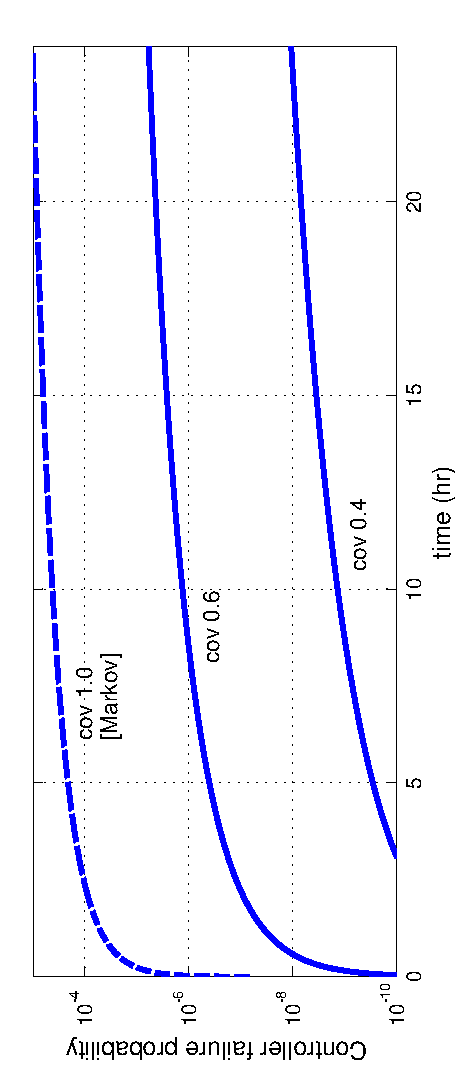
\includegraphics[scale=0.8, angle=-90]{DIComparison}
  \caption{Controller system failure probability comparing variability in time to previous-output.\label{fig:DIComparison}} 
\end{figure}

Figure \ref{fig:DIComparison} shows the controller failure probability for three cases of coefficient of variation: 1.0, 0.6 and 0.4. Recall that this variability corresponds to  time to the previous output from the state of correct output. Comparing the Figures \ref{fig:MarkovState3} and \ref{fig:DIComparison}, it can be seen that a cov of 1.0 reduces to the Markov case. On the other hand, lower the variability, lesser is the failure probability. 

\begin{table}[!h] \centering
\caption{Controller failure probability at the end of 24 hrs.\label{tbl:ControllerFailureProb}}
\begin{tabular}{ll}
\hline
$cov$ & Controller failure  \\
 & probability \\
\hline
1.0		&		1.0075 x $10^{-3}$ \\
0.6		&		5.88034 x $10^{-6}$ \\
0.4		&   1.05061 x $10^{-8}$ \\
\hline
\end{tabular}
\end{table}

The controller failure probabilities at the end of 24 hrs are shown in Table \ref{tbl:ControllerFailureProb} for each of the covs considered.  It is seen that the failure probability increases to 1.0075 x $10^{-3}$ when the time-to-previous output is relaxed to an assumption of exponential distribution, whereas if the actual cov had been  0.4, the probability is seen to be as low as 1.05061 x $10^{-8}$. 


\begin{figure}[h!] \centering
  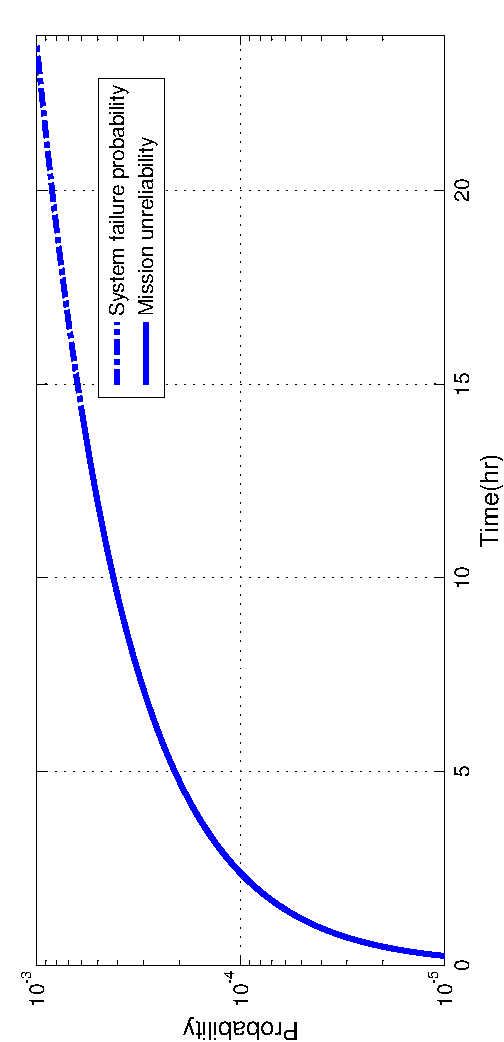
\includegraphics[scale=0.8, angle=-90]{DICMarkovMissionUnreliability}
  \caption{Controller system mission unreliability for additional 14 hrs given that the system was reliable for the initial 10 hrs [$cov$=1].\label{fig:DICMarkovMissionUnreliability}} 
\end{figure}

Since a digital I\&C system is a combination of hardware and software systems, it is prone to aging. 
Nuclear power plant systems are so highly sophisticated that certain maintenance activities could be carried out even without planned outages. Under these circumstances, continuous execution of software embedded in hardware (firmware) could exhibit software aging due to performance degradation, numerical error accumulation and unexpected crashes \citep{Linda2006}. Moreover, mechanical movement of the feedwater valve in response to controller commands could go out of control.


In an intuitive sense, the failure probability of an aging system at the present moment is very low given that the system was reliable until now. Overtime, failure probability of such a system is likely to be larger than that of a newly installed system due to increased risks of wear and tear. However both these quantities remain the same if the failure time of a system is assumed to follow an exponential distribution. This inability to take aging in to account is a result of the memoryless property of the exponential distribution as seen by comparing the system failure probability and the mission unreliability of the MFV controller with $cov=1$ in Figure \ref{fig:DICMarkovMissionUnreliability}. 

\begin{figure}[h!] \centering
  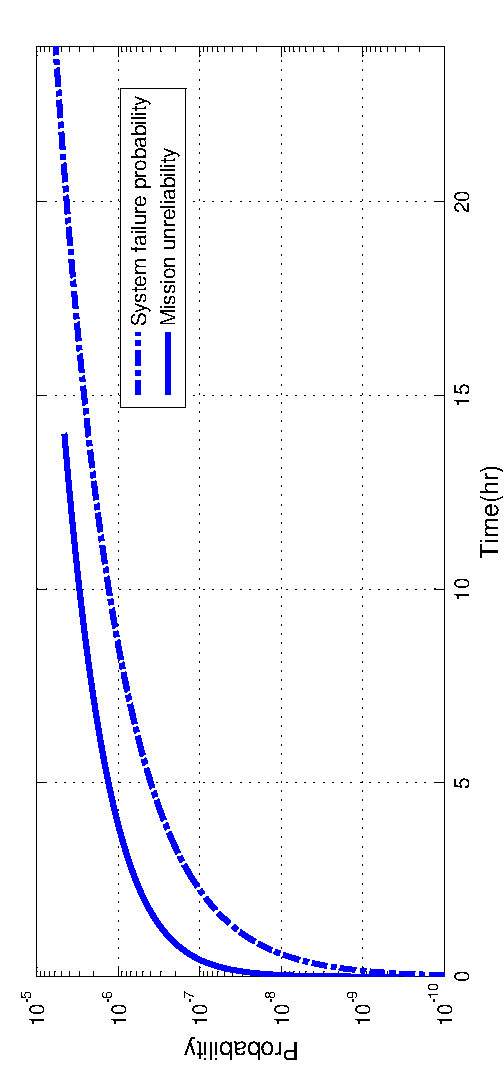
\includegraphics[scale=0.8, angle=-90]{DICSemiMarkovMissionUnreliability}
  \caption{Controller system mission unreliability for additional 14 hrs given that the system was reliable for the initial 10 hrs [$cov$=0.6].\label{fig:DICSemiMarkovMissionUnreliability}} 
\end{figure}

Assuming a $cov=0.6$ for the variability in the time to previous output, Figure \ref{fig:DICSemiMarkovMissionUnreliability} shows that mission unreliability of a system that survived 10 hrs is indeed larger than the system failure probability of a newly installed system.



Apart from the main feedwater regulating valve (MFV) controller, the digital feedwater controller system (DFWCS) is connected to a feedwater pump (FP) and its controller, a bypass feedwater valve (BFV) and its controller, a main computer and its backup and a pressure drop indicator (PDI) controller. A critical application in the nuclear plant reliability analysis is the probabilistic assessment of the entire digital controller system. NUREG-CR/6942 proposed Markov models for each of MFV, computer and the PDI systems. The MFV, BFV and the FP share the same model used in this paper. Hence, a larger application of semi-Markov process model would be to integrate the reliability models of the above said systems in to a single model for the digital feedwater controller system.


\section{Conclusion}
\label{sec:DICConclusion}
The main feedwater valve controller system used to regulate  water level in a nuclear power plant steam generator is a critical digital instrumentation and control system of interest. A Markov model developed based on NUREG-CR/6942 was extended to a semi-Markov model so that Weibull distribution could be assumed for the time-to-previous output from a correct output instead of an exponential distribution. The advantage of this approach is the ability to incorporate software and hardware aging in to the reliability model. The benefits have been demonstrated in this paper through time dependent system failure probability and mission unreliability results of the feedwater valve controller system. Better predictability of controller system reliability has a direct impact on probabilistic risk analysis of the entire Digital Feedwater Controller System (DFWCS).


%% The Appendices part is started with the command \appendix;
%% appendix sections are then done as normal sections
%\appendix



\section{Closed form solution for $W_i(t)$}

In this appendix, it is proved that a semi-Markov process model's kernel can be
entirely built using poly-Weibull distribution.

Let transition from a state $i$ to a state $j$ follow a poly-Weibull distribution
made of a mixture of $n$ Weibull distributions. If $n=1$, distribution
is a regular Weibull distribution. 


Consider a row $i$ whose entries represent  a competing risk situation, then for $1 \le j,k \le N$,


$\int\limits_0^t {\displaystyle\sum\limits_j {c_{ij} (t)dt} }$
\begin{align}
=& \int\limits_0^t{\sum\limits_j {[f_{ij}(t)\prod\limits_{k\ne j}{(1-F_{ik}(t))}]} dt} \nonumber \\
=&\int\limits_0^t {\sum\limits_j{[ \displaystyle\sum_{p=1}^{m_{ij}}(\lambda_{ijp} \gamma_{ijp}) (\lambda_{ijp}t)^{\gamma_{ijp}-1} e^{-\displaystyle\sum\limits_{k}\sum\limits_{q=1}^{m_{ik}}{(\lambda_{ikq}t)^{\gamma_{ikq}}}}   ]} dt} \nonumber \\
=&-e^{-X} + 1
\label{eqn:PolyWblIntegral}
\end{align}
where
\begin{align}
X =& \sum_{k}\sum_{q=1}^{m_{ik}}{(\lambda_{ikq}t)^{\gamma_{ikq}}}  \text{ so that} \nonumber \\
dX =& \sum_k\displaystyle\sum_{q=1}^{m_{ik}}(\lambda_{ijq} \gamma_{ijq}) (\lambda_{ijq}t)^{\gamma_{ijq}-1}dt \nonumber
\end{align}

The $W_i(t)$ in Integral Equation \ref{CTMRE} based on Equation \ref{eq:staying} is computed as
\begin{align}
W_i(t) = 1-(\ref{eqn:PolyWblIntegral})  = e^{-X} = e^{-\displaystyle\sum_{k}\sum_{q=1}^{m_{ik}}{(\lambda_{ikq}t)^{\gamma_{ikq}}}}
\label{eq:PolyWblStaying}
\end{align}
This simplified expression for $W_i(t)$ aids in fast computation of the state probabilities in the presence of
numerous competing risk situations.
It remains to plug-in both the matrices $C(t)$ and $W(t)$ and evaluate the state probabilities
recursively using Equation \ref{MatMRE} by applying the trapezoidal rule in Equation \ref{TrapCTMRE}.



\section{Implementation issues}
\label{sec:PipingImplementation}

Equation \ref{MatMRE} can be evaluated by direct numerical integration or using Laplace transforms method. Most distributions do not possess a closed form Laplace transform. \cite{Gulyas2007} in a thesis dissertation employed a transform approximation method (TAM) to evaluate the Laplace transform of Weibull distribution and then numerically evaluated its Laplace inversion. In this paper, we resort to the direct numerical integration technique since we assume that we do not know the degradation distribution beforehand.

Equation \ref{eq:staying} is computationally expensive if the integral has to be evaluated for each $t$. Instead, it can be computed as a recurrence relation as follows:

\begin{align}
W_i(t_n)=\begin{cases}
1 - \int_0 ^ {\Delta t} {w_i(t_n) dt} & n=1 \\
W_i(t_{n-1}) -\int_{t_{n-1}}^{t_n} { w_i(t) dt}    & n > 1
\end{cases}
\end{align}


Where, by trapezoidal rule, we have:

\begin{align}
\int_{t_{n-1}}^{t_n} {w_i(t)}dt = \frac{\Delta t}{2}\{  w_i(t_{n-1}) + w_i(t_n)  \} 
\end{align}

However, when all the failure/repair distributions follow Weibull distribution with scale $\lambda_{ik}$  and shape $\gamma_{ik}$, $W_i(t)$ reduces to a closed form as seen in the above Appendix:

\begin{align}
W_i(t) =  e^{-\sum\limits_{k}{(\lambda_{ik}t)^{\gamma_{ik}}}}
\end{align}

To solve the system of integral equations, \cite{Nunn1977} derived the following recurrence relation based on trapezoidal rule by distributing $t$ on a set of equally spaced points in the interval $[0,t]$:

\begin{eqnarray}
{\phi (t_n )} = [I - \frac{{\Delta t}}{2}C(0)]^{ - 1} [diag(W(t_n )) + \nonumber \\
\Delta t\sum\limits_{k = 1}^n {C(t_k ){\phi (t_n  - t_k )}}  - \frac{{\Delta t}}{2}C(t_n ){\phi (0)}]
\label{TrapCTMRE}
\end{eqnarray}

Where $\Delta t = t_n - t_{n-1}$. The solution is started with ${\phi(0)} = W(0) = I$.

The convolution operation in the above equation involves repeated addition and multiplication of matrices thus slowing down the computations as $n$ grows. With sufficiently large storage space, the following technique for convolution improves the speed:

\begin{align}
\sum\limits_{k = 1}^n C(t_k )&{\phi (t_n  - t_k )} = \nonumber \\
& \begin{bmatrix}
C(t_1) &  C(t_2) & ... & C(t_n)
\end{bmatrix}
 \begin{bmatrix}
{\phi(t_{n-1})} & {\phi(t_{n-2})} ... {\phi(t_0)}=I
\end{bmatrix}^T
\end{align}


\appendix



%\section{Closed form solution for $W_i(t)$}
%
%In this appendix, it is proved that a semi-Markov process model's kernel can be
%entirely built using poly-Weibull distribution.
%
%Let transition from a state $i$ to a state $j$ follow a poly-Weibull distribution
%made of a mixture of $n$ Weibull distributions. If $n=1$, distribution
%is a regular Weibull distribution. 
%
%
%Consider a row $i$ whose entries represent  a competing risk situation, then for $1 \le j,k \le N$,
%
%
%$\int\limits_0^t {\displaystyle\sum\limits_j {c_{ij} (t)dt} }$
%\begin{align}
%=& \int\limits_0^t{\sum\limits_j {[f_{ij}(t)\prod\limits_{k\ne j}{(1-F_{ik}(t))}]} dt} \nonumber \\
%=&\int\limits_0^t {\sum\limits_j{[ \displaystyle\sum_{p=1}^{m_{ij}}(\lambda_{ijp} \gamma_{ijp}) (\lambda_{ijp}t)^{\gamma_{ijp}-1} e^{-\displaystyle\sum\limits_{k}\sum\limits_{q=1}^{m_{ik}}{(\lambda_{ikq}t)^{\gamma_{ikq}}}}   ]} dt} \nonumber \\
%=&-e^{-X} + 1
%\label{eqn:PolyWblIntegral}
%\end{align}
%where
%\begin{align}
%X =& \sum_{k}\sum_{q=1}^{m_{ik}}{(\lambda_{ikq}t)^{\gamma_{ikq}}}  \text{ so that} \nonumber \\
%dX =& \sum_k\displaystyle\sum_{q=1}^{m_{ik}}(\lambda_{ijq} \gamma_{ijq}) (\lambda_{ijq}t)^{\gamma_{ijq}-1}dt \nonumber
%\end{align}
%
%The $W_i(t)$ in Integral Equation \ref{CTMRE} based on Equation \ref{eq:staying} is computed as
%\begin{align}
%W_i(t) = 1-(\ref{eqn:PolyWblIntegral})  = e^{-X} = e^{-\displaystyle\sum_{k}\sum_{q=1}^{m_{ik}}{(\lambda_{ikq}t)^{\gamma_{ikq}}}}
%\label{eq:PolyWblStaying}
%\end{align}
%This simplified expression for $W_i(t)$ aids in fast computation of the state probabilities in the presence of
%numerous competing risk situations.
%It remains to plug-in both the matrices $C(t)$ and $W(t)$ and evaluate the state probabilities
%recursively using Equation \ref{MatMRE} by applying the trapezoidal rule in Equation \ref{TrapCTMRE}.



%\section{Implementation issues}
%\label{sec:PipingImplementation}
%
%Equation \ref{MatMRE} can be evaluated by direct numerical integration or using Laplace transforms method. Most distributions do not possess a closed form Laplace transform. \cite{Gulyas2007} in a thesis dissertation employed a transform approximation method (TAM) to evaluate the Laplace transform of Weibull distribution and then numerically evaluated its Laplace inversion. In this paper, we resort to the direct numerical integration technique since we assume that we do not know the degradation distribution beforehand.
%
%Equation \ref{eq:staying} is computationally expensive if the integral has to be evaluated for each $t$. Instead, it can be computed as a recurrence relation as follows:
%
%\begin{align}
%W_i(t_n)=\begin{cases}
%1 - \int_0 ^ {\Delta t} {w_i(t_n) dt} & n=1 \\
%W_i(t_{n-1}) -\int_{t_{n-1}}^{t_n} { w_i(t) dt}    & n > 1
%\end{cases}
%\end{align}
%
%
%Where, by trapezoidal rule, we have:
%
%\begin{align}
%\int_{t_{n-1}}^{t_n} {w_i(t)}dt = \frac{\Delta t}{2}\{  w_i(t_{n-1}) + w_i(t_n)  \} 
%\end{align}
%
%However, when all the failure/repair distributions follow Weibull distribution with scale $\lambda_{ik}$  and shape $\gamma_{ik}$, $W_i(t)$ reduces to a closed form as seen in the above Appendix:
%
%\begin{align}
%W_i(t) =  e^{-\sum\limits_{k}{(\lambda_{ik}t)^{\gamma_{ik}}}}
%\end{align}
%
%To solve the system of integral equations, \cite{Nunn1977} derived the following recurrence relation based on trapezoidal rule by distributing $t$ on a set of equally spaced points in the interval $[0,t]$:
%
%\begin{eqnarray}
%{\phi (t_n )} = [I - \frac{{\Delta t}}{2}C(0)]^{ - 1} [diag(W(t_n )) + \nonumber \\
%\Delta t\sum\limits_{k = 1}^n {C(t_k ){\phi (t_n  - t_k )}}  - \frac{{\Delta t}}{2}C(t_n ){\phi (0)}]
%\label{TrapCTMRE}
%\end{eqnarray}
%
%Where $\Delta t = t_n - t_{n-1}$. The solution is started with ${\phi(0)} = W(0) = I$.
%
%The convolution operation in the above equation involves repeated addition and multiplication of matrices thus slowing down the computations as $n$ grows. With sufficiently large storage space, the following technique for convolution improves the speed:
%
%\begin{align}
%\sum\limits_{k = 1}^n C(t_k )&{\phi (t_n  - t_k )} = \nonumber \\
%& \begin{bmatrix}
%C(t_1) &  C(t_2) & ... & C(t_n)
%\end{bmatrix}
% \begin{bmatrix}
%{\phi(t_{n-1})} & {\phi(t_{n-2})} ... {\phi(t_0)}=I
%\end{bmatrix}^T
%\end{align}

  


%% References
%%
%% Following citation commands can be used in the body text:
%%
%%  \citet{key}  ==>>  Jones et al. (1990)
%%  \citep{key}  ==>>  (Jones et al., 1990)
%%
%% Multiple citations as normal:
%% \citep{key1,key2}         ==>> (Jones et al., 1990; Smith, 1989)
%%                            or  (Jones et al., 1990, 1991)
%%                            or  (Jones et al., 1990a,b)
%% \cite{key} is the equivalent of \citet{key} in author-year mode
%%
%% Full author lists may be forced with \citet* or \citep*, e.g.
%%   \citep*{key}            ==>> (Jones, Baker, and Williams, 1990)
%%
%% Optional notes as:
%%   \citep[chap. 2]{key}    ==>> (Jones et al., 1990, chap. 2)
%%   \citep[e.g.,][]{key}    ==>> (e.g., Jones et al., 1990)
%%   \citep[see][pg. 34]{key}==>> (see Jones et al., 1990, pg. 34)
%%  (Note: in standard LaTeX, only one note is allowed, after the ref.
%%   Here, one note is like the standard, two make pre- and post-notes.)
%%
%%   \citealt{key}          ==>> Jones et al. 1990
%%   \citealt*{key}         ==>> Jones, Baker, and Williams 1990
%%   \citealp{key}          ==>> Jones et al., 1990
%%   \citealp*{key}         ==>> Jones, Baker, and Williams, 1990
%%
%% Additional citation possibilities
%%   \citeauthor{key}       ==>> Jones et al.
%%   \citeauthor*{key}      ==>> Jones, Baker, and Williams
%%   \citeyear{key}         ==>> 1990
%%   \citeyearpar{key}      ==>> (1990)
%%   \citetext{priv. comm.} ==>> (priv. comm.)
%%   \citenum{key}          ==>> 11 [non-superscripted]
%% Note: full author lists depends on whether the bib style supports them;
%%       if not, the abbreviated list is printed even when full requested.
%%
%% For names like della Robbia at the start of a sentence, use
%%   \Citet{dRob98}         ==>> Della Robbia (1998)
%%   \Citep{dRob98}         ==>> (Della Robbia, 1998)
%%   \Citeauthor{dRob98}    ==>> Della Robbia


%% References with bibTeX database:
%\bibliographystyle{model2-names}
\bibliographystyle{elsarticle-harv}

% This specifies the location of the file containing the bibliographic information.  It assumes you're using BibTeX (if not, why not?).
\bibliography{uw-ethesis}
% Tip 5: You can create multiple .bib files to organize your references. 
% Just list them all in the \bibliogaphy command, separated by commas.
%\nocite{*}

%\begin{thebibliography}{14}
%\end{thebibliography}



\end{document}
